% ######################################################################################################################
%         Foundations
% ######################################################################################################################

\chapter{Foundations}
\label{ch:Foundations}

\paperbox{
    This chapter is partially based on the peer-reviewed publications:
}{\paperart \paperpppp}{
    \todo{
        \textbf{Contributions:} Lucas Czech... Pierre Barbera... Alexandros Stamatakis... and...
    }
}

\todo{In this chapter, we introduce\ldots}

% ######################################################################################################################
%         Evolution and Genetics
% ######################################################################################################################

\section{Evolution and Genetics}
\label{ch:Foundations:sec:EvolutionGenetics}

% Evolution is change in the heritable characteristics of biological populations over successive generations.
% \url{https://en.wikipedia.org/wiki/Evolution}
% the process by which new species or populations of living things develop from preexisting forms through successive generations
% \url{https://www.merriam-webster.com/dictionary/evolution}
% Evolution is a process of continuous branching and diversification from common trunks. This pattern of irreversible separation gives life's history its basic directionality. —Stephen Jay Gould
% \url{https://www.merriam-webster.com/dictionary/evolution}

% Evolution is the continuous process of diversification of biological populations through successive generations \cite{Hall2008}.

Life on Earth is at least 3.77 billion years old \cite{Dodd2017},
and is continuously evolving due to \emph{natural selection} \cite{Darwin1859}.
% Woah, I like that very first sentences. A very old and a very new publication, binding all of reasearch together...
Driven by \emph{variation}, biological populations diversify through successive generations,
leading to the origination of new species.
This continuous process is called \emph{evolution} \cite{Hall2008}.
Heritable characteristics are passed down from parent to offspring,
with occasional random mutations leading to variation.
Thus, some organisms are better adapted to their environment than others,
and have more reproductive success.
There is hence a natural selection for advantageous mutations,
which can then spread through generations.

% this process was not understood for a long time. static species?
% four driving forces of pop gen?

The characteristics and traits of an organism are carried by, and inherited via, \emph{deoxyribonucleic acid} (DNA).
DNA is the molecule that encodes the genetic information needed for the functioning of all living organisms.
It is structured in form of a double helix \cite{Watson1953},
and built from two strands of molecules called \emph{nucleotides}.
The nucleotides build the backbone of the double helix,
and connect the two strands via opposing pairs of \emph{nucleobases}.
The redundant structure of pairs of nucleobases gives stability to the DNA molecule,
and also serves as a mechanism of error correction when reading the genetic information.
% both of which is important for the role of DNA for information storage.
In DNA, there are four distinct nucleobases:
adenine (\nba), cytosine (\nbc), guanine (\nbg), and thymine (\nbt),
where \nba pairs with \nbt, and \nbc pairs with \nbg, respectively.

The sequence of nucleobases along the strands of DNA is what encodes the genetic instructions
used by all known living organisms.
Parts of the DNA encode for proteins,
which perform a plethora of different functions within organisms.
Proteins consist of long chains of amino acid residues, and
are assembled in a process called protein (bio)synthesis.
This is described by the central dogma of molecular biology \cite{Crick1958,Crick1970}:
First, DNA is \emph{transcribed} into the intermediary ribonucleic acid (RNA),
which is then \emph{translated} into the actual protein.

In each step of this process, the alphabet used to encode information differs.
While DNA uses the four nucleobases as described above,
in RNA, the nucleobase uracil (\nbu) is used instead of thymine (\nbt).
Proteins on the other hand are (mostly) build from a set of \num{20} standard amino acids.
The set of rules for translating nucleobases into amino acids is called the \emph{genetic code}:
In a DNA sequence, three consecutive nucleobases are needed to encode one amino acid.

The entirety of the genetic material of an organism, that is, its complete DNA sequence, is called its \emph{genome}.
A \emph{gene} is a sequence which codes for a molecule that has a particular function, such as a protein \cite{Gericke2007}.
DNA and genes are the basic units of heredity.
They are what is varying across generations,
and what is selected for in the process of natural selection \cite{Dawkins1989}.
The study of genes, variation and heredity is called \emph{genetics} \cite{Griffiths2000}.

All life on this planet is related to each other and descends from a common ancestor.
Still, it is remarkable that the basic molecular principles and mechanisms of life
-- DNA, amino acids, and the genetic code -- are virtually identical for all living organisms.
This implies that by understanding and comparing the genetic information encoded in the DNA of different organisms,
one can understand the diversification patterns of evolution.

% ######################################################################################################################
%         Sequence Analysis
% ######################################################################################################################

\section{Sequence Analysis}
\label{ch:Foundations:sec:SequenceAnalysis}

% ======================================================================================================================
%     Genome Sequencing
% ======================================================================================================================

\subsection{Genome Sequencing}
\label{ch:Foundations:sec:SequenceAnalysis:sub:GenomeSequencing}

Prior to analyzing the DNA of an organism, the physical order of nucleobases in the DNA molecule has to be determined.
That is, the DNA has to be ``read'' and stored in a human-accessible text format, typically a computer file.
This technical process is called DNA \emph{sequencing}.
% which can be understood as putting biomass into a blender and converting it into text files ;-)

For many decades, the main technique for this purpose was Sanger sequencing \cite{Sanger1975,Sanger1977}.
It is labor- and time-intensive, but through improvement and automation, costs were constantly reduced.
Eventually, this allowed for large-scale efforts, such as the Human Genome Project \cite{Venter2001},
which sequenced the whole human genome of more than three billion nucleobases.
Sanger sequencing allows to determine long parts of the sequence at once (> \num{500} nucleobases),
which then have to be assembled to build the final sequence.

In the last decades, a variety of novel high-throughput DNA sequencing technologies
have been developed \cite{Pettersson2009,Reuter2015,Deiner2017b}.
In particular, \emph{Next Generation Sequencing} (NGS) \cite{Logares2012,Mardis2013}
has revolutionized biology by transforming it into a data-driven and compute-intense discipline \citep{Escobar-Zepeda2015}.
The costs of these technologies are decreasing faster than Moore's law \cite{Wetterstrand2018}.
This leads to a ``tsunami'' of sequence data,
which poses a challenge for computational methods working with these data.
Compared to Sanger sequencing, NGS technologies are generally cheaper and faster \cite{Voelkerding2009,Metzker2010},
but come at the price of introducing more errors in the sequence output,
or only being able to determine shorter parts of the sequence at once
-- both of which constitute a challenge for the subsequent assembly of the final sequence.

The result of DNA sequencing is a textual representation of the order of nucleobases.
Each contiguous sequence coming from the sequencing machine is called a \emph{read}.
Because of the pairing of nucleobases,
both DNA strands can be sequenced, which provides a means of error correction.
Such data are typically stored in the \fileformat{fastq} file format \citep{Cock2009}.
These so-called paired-end reads are then merged to form a final sequence representation of one strand
% cite \toolname{PEAR} \cite{Zhang2014} ?
-- that is, a sequence of the characters \nba, \nbc, \nbg, and \nbt.
These data are stored in formats such as the \fileformat{fasta} file format \citep{Pearson1988}.
Due to the pairing of nucleobases,
the length of a DNA sequence is measured in \emph{base pairs} (abbreviated \si{\basepair}):
\SI{1}{\basepair} represents one character in the file.
These files are then the input for computational methods for working with DNA sequences.

% Not needed right now:
% Because of the universal genetic code of translating DNA to amino acids,
% it is also possible to store the amino acid sequence instead of the nucleobase sequence.

% ======================================================================================================================
%     Metagenomics
% ======================================================================================================================

\subsection{Metagenomics}
\label{ch:Foundations:sec:SequenceAnalysis:sub:Metagenomics}

Sanger sequencing requires careful preparation of the genetic material,
and is thus best used for sequencing single organisms.
There are however many (microbial) organisms that cannot be cultured in a Petri dish,
and are hence hard to sequence with this technique.
Apart from being cheaper, Next Generation Sequencing machines however ``digest'' all genetic material presented to them.
They thus allow for studying microbial samples
directly extracted from their environment \citep{Morgan2010,Edwards2013,Sunagawa2013a}.
This enables to study environments such as
water \cite{Karsenti2011,Giner2016,Gran-Stadniczenko2017},
soil \cite{Dupont2016,Mahe2017},
the human body \cite{Huttenhower2012,Methe2012,Srinivasan2012,Matsen2015},
and many others.
Each sample from such an environment then represents a geographical location, a body site, a point in time, etc.
% These studies yield a large set of short anonymous DNA reads for each sample.
% The DNA reads obtained from sequencing a sample represent all organisms present in the sample;
The DNA of all organisms being present in a sample is sequenced,
resulting in a large number of reads per sample.
These reads are anonymous, as it is unclear to which organism they originally belonged.

The study of these data, that is, genetic material from environmental samples, is called \emph{metagenomics} \cite{Oulas2015}.
% A first step is often to generate a genetic profile of the environment,
% that is, to estimate the diversity of the organisms in the sample.
A first step in such studies is often to characterize the reads obtained from an environment
in terms of \emph{reference sequences} of known species.
Reads that are similar to (parts of) reference sequences can be assigned to them,
while reads with low similarity to known sequences might indicate novel, undescribed species \cite{Temperton2012}.
Key tasks in metagenomic studies are the identification and classification of the anonymous reads (``Who is there?''),
and their functional annotation (``What are they doing?'') \cite{Desai2012}.
Both are introduced in the following.

% The following paragraph is not totally needed, as we are not doing functional analysis.
% However, it introduces many other terms alongside, which is useful later on.
Functional annotation \cite{Stein2001} is the prediction of gene functions of the reads,
and the inference of metabolic capacity of microbial communities \cite{Brown2017}.
As the proteins that are needed in the pathways of such functions can be encoded by genes across the genome,
whole-genome sequencing is necessary to capture all genes of interest.
For example, in shotgun sequencing \cite{Staden1979,Anderson1981},
the DNA is fragmented into small pieces within the size range that the used sequencing technology can handle,
typically a few hundred \si{\basepair} long.
This allows to sequence all genetic material contained in a sample.
Thus, the resulting reads originate from different parts of the genomes of their organisms,
which can then be functionally annotated \cite{Glass2010}.
This however necessitates to use whole-genome reference sequences
in order to be able to assign reads to known species and functions.
Typical databases of reference sequences however
lack many of the protein sequences from the microbial species present in a sample,
mostly because of organisms that cannot be cultured \cite{Brown2017}.

For the task of identification and classification of reads however, whole genome references are not needed.
Instead, specific \emph{marker genes} can be used,
which are regions of genes that are particularly suited for delineating between different species \cite{Ren2016}.
% highly conserved, that is, slowly changing over evolutionary times.
% but certain parts are radpidly evolung (hyper variable) withing the region, which is good for delineation.
% typically, this is general basic cell functionen stuff, which is needed by many forms of live.
% eg cell division, ssu... mitochondrial dna, etc
The method of using marker genes to identify species is called \emph{DNA barcoding} \cite{Hebert2003,Savolainen2005}.
The choice of genes to use as marker is important, and depends on the types of organisms to be studied.
The used marker genes should ideally be present in (most of) the organisms of interest,
short enough to be sequenced with current technology,
and have enough variation between species to distinguish between them,
but have low variation within species \cite{Kress2008}.

In many metagenomic studies of \taxonname{bacteria} and \taxonname{eukaryotes},
the 16S \cite{Weisburg1991} and 18S \cite{Meyer2010} rRNA regions are used as marker genes,
respectively \cite{Woese1977,Woese1990}.
These regions belong to the small subunit (SSU) of the ribosomal ribonucleic acid (rRNA),
which is an essential component of the ribosome.
The ribosome is a molecular machinery that is responsible for protein synthesis (translation) in all living organisms.
% and are thus present in virtually all \taxonname{bacteria} and \taxonname{eukaryotes}.
Often, prior to sequencing, these regions are amplified by many orders of magnitude,
using polymerase chain reaction (PCR) to create copies of these regions \cite{Bartlett2003}.
The resulting reads are then de-replicated again, which results in sequences called \emph{amplicons}.
While the PCR amplification process is known to introduce bias \cite{Logares2014},
this method is commonly used, particularly for the 16S and 18S rDNA regions.
Hence, many databases provide reference sequences for these regions.
The amplicons can then be employed to estimate the microbial diversity of the organisms in a sample
by comparison against known species.

% Not needed right now:
% from \cite{Brown2017}:
% Measurement of the taxonomic composition of metagenome samples by PCR and
% amplicon sequencing of the 16S rDNA marker gene is inexpensive, but it is subject to bias and lacks
% sensitivity below the species level.
%
% thus, a recent technique: mi tags \cite{Logares2014}
% where specific sequences of a wgs approach are filtered to only contain reads from marker regions

% ======================================================================================================================
%     Sequence Alignments
% ======================================================================================================================

\subsection{Sequence Alignment}
\label{ch:Foundations:sec:SequenceAnalysis:sub:SequenceAlignment}

When comparing sequences to each other, it is important to know which characters are \emph{homologous},
that is, evolved from the


pairwise alignment section

review of msa software \cite{Thompson2011}

show unaligned sequences and an alignment. maybe show consensus sequence, too, for next section.

only makes sense when evlultionary related. thus, for distantly related species, often conserved regions are used,
eg 16s 18s, or barcodes or stuff


introduce ``indels'' and homologous chars, orthologous genes, etc

\figref{fig:msa} shows an example of the process and the resulting MSA.

\begin{figure}[hpbt]
    \centering
%     \vspace*{0.5em}
    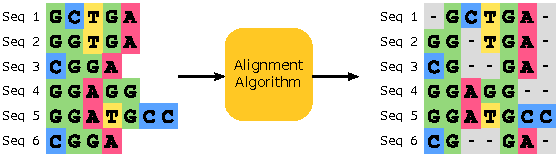
\includegraphics[width=.9\linewidth]{msa.pdf}
    \caption[Multiple Sequence Alignment]{
        \textbf{Multiple Sequence Alignment.}
        The left hand side shows a set of six sequences.
        Using an alignment algorithm, gaps are inserted into these sequences at presumed \emph{indel} positions.
        The right hand side shows the result of this process,
        where homologous characters in the columns of the multiple sequence alignment (MSA) are aligned to each other.
    }
    \label{fig:msa}
\end{figure}

% ======================================================================================================================
%     Consensus Sequences
% ======================================================================================================================

\subsection{Consensus Sequences}
\label{ch:Foundations:sec:SequenceAnalysis:sub:ConsensusSequences}

maybe move to PhAT, as this is not relevant for the other chapters,
and not for the introduction in general.

ambiguity chars \cite{IUPAC1971}

cons methods: see art

% ######################################################################################################################
%         Tree of Life
% ######################################################################################################################

\section{The Tree of Life}
\label{ch:Foundations:sec:TreeOfLife}

maybe move to trees:

all use the same or very similar mechanisms, dna, genetic code etc are (almost) universal throughout life.
this suggests that there is common decent.

branching pattern, common decent, etc leads naturally to a tree structure
(ignoring the messiness of biology)

there is common functionality - the closer related two organisms are in evolutionary terms,
the more similarities are to be expected in their dna.

Given that all life is related by its evolutionary history,
a key question is how these relationtions are

that is, comaring sequenes, finding tree of life

what is a species.

% ======================================================================================================================
%     Taxonomy and Nomenclature
% ======================================================================================================================

\subsection{Taxonomy and Nomenclature}
\label{ch:Foundations:sec:TreeOfLife:sub:TaxonomyNomenclature}

there is more than one species on Earth [citation needed]. also, evolution naturally gives rise to a branching pattern,
which can be interpreted as a hierarchy. higher levels represent common ancestors

sort organisms into categories, eg Aristotle
historically: morphology based: how does stuff look?

this is called taxonomy.
entries in a taxonomy have names, which follow a certain nomenclature, e.g. Lineaus
introduce ``taxon'' (plural ``taxa'') as well here.

highest level: three domains model.
bact arch euks.

the lower levels in the tax usually represent species or even strains (\eg of bacteria).

now: genes and dna used more and more to refine the taxonomy of life.

% ======================================================================================================================
%     Phylogenetics
% ======================================================================================================================

\subsection{Phylogenetics}
\label{ch:Foundations:sec:TreeOfLife:sub:Phylogenetics}

phylogenetics is...

in context of trees, the sequences are thought to represent species, or \emph{taxa} that one is interested in.
introduce ``taxa'', ref to tax intro above

show a tree. maybe darwin?
idea: trees show evol relationships. closer in the tree, closer in evol.
branch lengths etc.

not considering lat gene tranfs,
there is only one ``true'' tree of life.

% ======================================================================================================================
%         Tree Inference
% ======================================================================================================================

\subsection{Tree Inference}
\label{ch:Foundations:sec:TreeOfLife:sub:TreeInference}


but, no time machine, fuzzy and missing data, etc. so we have to infer as well as possible from the given data.
that is, methods to mathematically model evolution.
in other words, from all possible trees, we want to find one that is good

for a given number of taxa $n$, the number of distinct tree topologies N is given as
$N(n) = \prod_{i=3}^{n} (2i - 5)$
grows over-exponentially fast
\cite{Felsenstein2004}

tree search, number of trees, more than exp. effort

inference can be interpreted as a search in the space of all possible trees for the tree that maximizes some optimality criterion.

also, we can infer trees \cite{Felsenstein2004}

\cite{Yang2006}


space is large, so there are different approaches and heuristics to inferring trees.


Distance based methods such as \emph{Unweighted Pair Group Method with Arithmetic Mean} (UPGMA) \cite{Sokal1958}
and \emph{Neighbor Joining} \cite{Saitou1987}
use a pairwise distance matrix between sequences, and thus do not necessarily need an alignment.
\emph{Maximum Parsimony} \cite{Sankoff1975} uses an optimality criterion that is based on Occam's razor,
that is, it yields the tree that explains the observed tip sequences (taxa)
with the minimal number of substitutions (mutations).
Furthermore, there is \emph{Bayesian Inference},
in which Bayes' theorem is used to calculate the posterior distribution of the relevant evolutionary processes,
and which thus can incorporate prior empirical knowledge into the process.

Bayesian approaches, ...

In the context of this work, we are mostly interested in Maximum Likelihood (ML) tree inference,
which is introduced below.

ML, baysian...

we here focus on ML.

subst models
% and thereafter evaluating the resulting likelihood score of the tree under a given model of nucleotide evolution,
% such as the Generalized Time-Reversible (GTR) model \cite{Tavare1986}.

ML grundidee

\begin{equation}
    L(~ \mbox{MSA} ~|~ T, \bar{b}, M, \bar{\theta} ~)
\end{equation}



tree properties, BL, node names, etc

BL opt

introduce ``phylogenetic signal''

explain visualizations, and that they are just a layout choice

tree formats?
newick etc

% ######################################################################################################################
%         Phylogenetic Placement
% ######################################################################################################################

\section{Phylogenetic Placement}
\label{ch:Foundations:sec:PhylogeneticPlacement}

introduce ``reference tree'', as a tree inferred from reference sequences.

. common use case: fixed tree, selected by experts to consist of know, described taxa
to represent the diversity expected from an environment.


Since the amount of sequence data produced in metagenomic studies can be quite substantial,
computational challenges and bottlenecks arise \cite{Scholz2012}.


% ======================================================================================================================
%     Motivation
% ======================================================================================================================

\subsection{Motivation}
\label{ch:Foundations:sec:PhylogeneticPlacement:sub:Motivation}


problem with ngs data:
msa is NP-hard \cite{Just2001}.
inferring tree for this many sequences is also NP-hard \cite{Chor2005} even harder (over exp.), plus
short sequences (not phylo signal), so cannot resolve relationtips between sequences


% although the methods generally are applicable to both.
A typical task in metagenomic studies is to identify and classify these sequences with respect
to known reference sequences, either in a taxonomic or phylogenetic context.
% another typical task: to discover novel diversity. not here.

Conventional methods like \toolname{Blast} \cite{Altschul1990} are based on sequence similarity.
Such methods are fast, but only attain satisfying accuracy levels
if the query sequences (e.g., the environmental reads or amplicons) are sufficiently similar to the reference sequences.
Furthermore, the best \toolname{Blast} hit does often \emph{not} represent the most closely related species \cite{Koski2001}.
% \todo{Mention further methods here, for example Vervier 2015}
This is particularly true for environments where available reference databases
do not exhibit sufficient taxon coverage \citep{Mahe2017}.
As insufficient taxon coverage cannot be detected by methods that are based on sequence similarity,
they can potentially bias downstream analyses.

Alternatively, so-called phylogenetic (or evolutionary) placement methods \cite{Matsen2010,Berger2011,Barbera2018}
identify query sequences based on a phylogenetic tree of reference sequences.
Thereby, they incorporate information about the evolutionary history of the species under study
and hence provide a more accurate means for read identification.
The result of phylogenetic placement is a mapping of the query sequences to the branches of the reference tree.
Such a mapping also elucidates the evolutionary distance between the query and the reference sequences.

This information represents useful biological knowledge \emph{per se}.
For example, the classification of query sequences can be summarized by means of sequence abundances \cite{Pace1997,Hugenholtz1998},
or to obtain taxonomic annotations \cite{Kozlov2016}.
The data can also be utilized to derive further knowledge or hypotheses.
Existing methods such as Edge PCA and Squash Clustering \cite{Matsen2011a} are, for instance, able
to visualize differences between sets of metagenomic samples,
or to cluster samples based on placement similarity.
Note that distinct samples from one study are typically mapped to the same underlying reference tree,
thus facilitating such comparisons.



phylogenetic placement \cite{Matsen2010,Berger2011,Barbera2018}, cited more than 630 times (as of 2018-07-01)
considered an established method

There also exist variants of phylogenetic placement that use maximum parsimony \cite{Berger2011}
and minimum evolution \cite{Filipski2015} instead of maximum likelihood,
variants that calculate Bayesian posterior probabilities \cite{Matsen2010},
and boosting methods to improve the accuracy of the placements \cite{Mirarab2012}.
Phylogenetic placement has been used for a variety of applications and derived pipelines, such as
species delimitation \cite{Zhang2013,Kapli2017},
genome and metagenome analysis \cite{Darling2014},
taxonomic identification and phylogenetic profiling \cite{Nguyen2014}, and
identification and correction of taxonomically mislabeled sequences \cite{Kozlov2016}.

combine 1,010 more citations (as of 2018-07-01)
see also recent art version

there is also a recent approach that yields comparable results (also jplace), but uses an alignment-free, non ML approach \cite{Linard2018}.


aligning

kommt unten noch mal!

, using programs such as \toolname{PaPaRa} \citep{Berger2011a,Berger2012} or
\toolname{hmmalign}, which is a subprogram of the \toolname{HMMER} suite \citep{Eddy1998,Eddy2009}.

% ======================================================================================================================
%     Introduction
% ======================================================================================================================

\subsection{Introduction}
\label{ch:Foundations:sec:PhylogeneticPlacement:sub:Introduction}

\todo{pipeline diagram, data flow, etc, reference to chapters?!}

In brief, phylogenetic placement calculates the most probable insertion branches for each given \acf{QS} on a \acf{RT}.
The \acp{QS} are reads or amplicons from environmental samples; most often barcoding regions or marker genes are used.
The \ac{RT} and the reference sequences it represents are typically assembled by the user
so that they capture the expected species diversity in the samples.
Nonetheless, we recently presented an automated approach
for selecting and constructing appropriate reference sequences from large sequence databases \cite{Czech2018}.
As phylogenetic placement used a maximum likelihood criterion, the \ac{RT} has to be strictly bifurcating.
Prior to the placement, the \acp{QS} need to be aligned against the reference alignment of the \ac{RT} by programs such as
\toolname{PaPaRa} \cite{Berger2011a,Berger2012} or
\toolname{hmmalign}, which is part of the \toolname{HMMER} suite \cite{Eddy1998,Eddy2009}.
The placement is then conducted by initially inserting one \ac{QS} as a new tip into a branch of the tree,
then re-optimizing the branch lengths that are most affected by the insertion,
and thereafter evaluating the resulting likelihood score of the tree under a given model of nucleotide evolution,
such as the Generalized Time-Reversible (GTR) model \cite{Tavare1986}.
The \ac{QS} is then removed from the current branch and subsequently placed into all other branches of the \ac{RT}.

Thus, for each branch of the tree, the process yields a so-called \emph{placement} of the \ac{QS},
that is, an optimized position on the branch, along with a likelihood score for the whole tree.
The likelihood scores for a \ac{QS} are then transformed into probabilities,
which quantify the uncertainty of placing the sequence on the respective branch \cite{Strimmer2002,VonMering2007}.
Those probabilities are called \acp{LWR}.
The accumulated \ac{LWR} sum over all branches for a single \ac{QS} is $1.0$.
\figref{fig:tree_epa} shows an example depicting the placements of one \ac{QS}, including the respective \acp{LWR}.

\begin{figure}[hpbt]
    \centering
    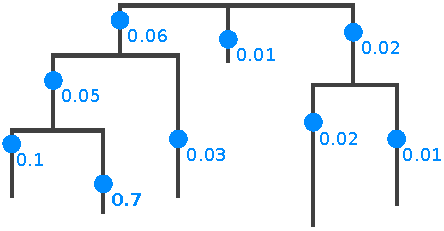
\includegraphics[width=.6\linewidth]{pppp/tree_epa.pdf}
    \caption[Phylogenetic Placement of a Query Sequence]{
        \textbf{Phylogenetic Placement of a Query Sequence.}
        Each branch of the reference tree is tested as a potential insertion position, called a ``placement'' (blue dots).
        Note that placements have a specific position on their branch, due to the branch length optimization process.
        A probability of how likely it is that the sequence belongs to a specific branch is computed
        (numbers next to dots),
        which is called the \emph{likelihood weight ratio} (LWR).
%         based on the maximum likelihood score of the whole tree. %(that is, including the query sequence)
        The bold number (0.7) denotes the most probable placement of the sequence.
    }
    \label{fig:tree_epa}
\end{figure}

This process is repeated for every \ac{QS}.
Note that the placement process is conducted {\em independently} for each \ac{QS}.
% Shorter: This placement process is conducted independently for each sequence.
That is, for each \ac{QS}, the algorithm starts calculating placements from scratch on the original \ac{RT}.
%This enables parallelization,
%and avoids unstable trees, which might result from adding too many sequences of short length to the tree.

In summary, the result of a phylogenetic placement analysis is a mapping of the \acp{QS} in a sample
to positions on the branches of the \ac{RT}.
Each such position, along with the corresponding \ac{LWR}, is called a placement of the \ac{QS}.
% The result of phylogenetic placement is a mapping of each \ac{QS} (e.g., environmental reads)
% to positions on the branches of the \ac{RT}, amended by probabilities in form of their likelihood weight ratios.
% Each \ac{QS} is thus represented by its placement positions, which are also called its placements.
% along with the respective likelihood weight ratios.f
% total: sum up. placement profile. imbalance. explain in later chapter.
% Here, we use these sample profiles to discover: clusters, correlation with meta-data.

\todo{besser unterbringen}
The data is usually stored in so-called \fileformat{jplace} files \cite{Matsen2012}.

% Each such sample represents a geographical location, a body site, a point in time, etc.
In the following, we represent a sample by the placement locations of its metagenomic \acp{QS},
including the respective per-branch \acp{LWR}.
Furthermore, for a specific analysis, we assume the standard use case,
that is, all placements were computed on the same fixed \acf{RT} and \acl{RA}.


This mapping can be seen as an identification and classification of the \acp{QS} in terms of the \ac{RT},
similar to a taxonomic assignment.
However, phylogenetic placement also allows for more elaborate downstream analyses.
Firstly, the reference tree usually offers a higher resolution than simple per-taxon abundance counts,
and the amount of mapped \acp{QS} per branch can be directly visualized on the \ac{RT} \citep{Mahe2017}.
Secondly, established methods such as Edge PCA and Squash Clustering \citep{Matsen2011a}
allow for identifying subtle differences between distinct samples,
thus enabling comparative studies directly based on phylogenetic placement.
Lastly, we recently proposed novel methods for visualizing and clustering phylogenetic placement data \citep{Czech2018a},
which, for example, can reveal correlations of per-sample meta-data features with sequence abundances.


Furthermore, phylogenetic placement is used in a variety of derived tools,
such as \toolname{(m)PTP} (species delimitation; \cite{Zhang2013,Kapli2017}),
\toolname{SEPP} (boosting; \cite{Mirarab2012}),
\toolname{PhyloSift} (metagenome analysis; \cite{Darling2014}),
\toolname{Sativa} (identification and correction of taxonomically mislabeled sequences; \cite{Kozlov2016})
and \toolname{TIPP} (taxonomic identification and phylogenetic profiling; \cite{Nguyen2014}).

A phylogenetic placement can be carried out {\em if} the \acp{QS} can be aligned to the reference alignment.
Often, barcoding regions such as 16S or 18S are used,
but there also exist studies that use different, or even a set of, maker genes \citep{Sunagawa2013a}.
Furthermore, other types of sequences such as $_{\text{mi}}$tags %\textsubscript{mi}tags
\citep{Logares2014} can be used.

% ======================================================================================================================
%     Placement Pipeline
% ======================================================================================================================

\subsection{Placement Pipeline}
\label{ch:Foundations:sec:PhylogeneticPlacement:sub:PlacementPipeline}


alignting against given ref aln, papara, hmmer

ML method, rappas (aln free)


% ######################################################################################################################
%         Phylogenetic Placement Processing
% ######################################################################################################################

\section{Phylogenetic Placement Processing}
\label{ch:Foundations:sec:PhylogeneticPlacementProcessing}

% thus, wehn dealing with many samples, an imporatn question is how to make them comparable when differing numbres o sequences
% the problem arises because different samples zies. can span many order sof magnitude.
When placing multiple samples, for instance, from different locations,
typically, the same \ac{RT} is used, in order to allow for comparisons of the phylogenetic composition of these samples.
In this context, it is important to consider how to properly normalize the samples.
Normalization is required as the sample size (often also called library size),
that is, the number of sequences per sample, can vary by several orders of magnitude,
due to efficiency variations in the sequencing process or biases introduced by the amplification process.
Selecting an appropriate normalization strategy constitutes a common problem in many metagenomic studies.
The appropriateness depends on data characteristics \cite{Weiss2017}, but also on the biological question asked.
For example, estimating indices such as the species richness are often implemented
via rarefaction and rarefaction curves \cite{Gotelli2001},
which however ignores a potentially large amount of the available valid data \cite{McMurdie2014}.
Furthermore, the specific type of input sequence data has to be taken into account for normalization:
Biases induced by the amplification process can potentially be avoided if, instead of amplicons,
data based on shotgun sequencing are used, such as \textsubscript{mi}tags \cite{Logares2014}.
Moreover, the sequences can be clustered prior to phylogenetic placement analysis,
for instance, by constructing operational taxonomic units (OTUs) \cite{Edgar2010,Mahe2014,Mahe2015,Rognes2016}.
Analyses using OTUs focus on species diversity instead of simple abundances.
OTU clustering substantially reduces the number of sequences,
and hence greatly decreases the computational cost for placement analyses.
Lastly, one may completely ignore the abundances (which are called ``multiplicities'' of placements) of the placed
sequences, reads, or OTUs, and only be interested in their presence/absence when comparing samples.

Which of the above analysis strategies is deployed,
depends on the specific design of the study and the research question at hand.
The common challenge is that the number of sequences per sample differs, which affects most post-analysis methods.
Before introducing our methods,
we therefore explain how the necessary normalizations of sample sizes can be performed in the following.
We also describe general techniques for interpreting and working with phylogenetic placement data.
%These are not methods of their own, but tools necessary for later.
Some of these techniques have been used before as building blocks
for methods like Edge PCA and Squash Clustering \cite{Matsen2011a,Evans2012}. \todo{see below}
%and we mostly stick to established terminology.

% ======================================================================================================================
%     Edge Masses
% ======================================================================================================================

\subsection{Edge Masses}
\label{ch:Foundations:sec:PhylogeneticPlacementProcessing:sub:EdgeMasses}

Methods that compare samples directly based on their sequences,
such as the UniFrac distance \cite{Lozupone2005,Lozupone2007a},
can benefit from rarefaction \cite{Weiss2017}.
However, in the context of phylogenetic placement, rarefaction is not necessary.
Thus, more valid data can be kept.
% Directly comparing individual anonymous sequences can be too computationally demanding for large contemporary metagenomic datasets.
% hence, the quantitative methods we present here do not consider the \acp{QS} individually.
% as contemporary metagenomic datasets are often too large to allow for this level of granularity,
To this end, it is convenient to think of the reference tree as a graph
(when exploiting graph properties of the tree, we refer to the branches of the tree as edges).
Then, the per-branch \acp{LWR} for a single \ac{QS}
can be interpreted as mass points distributed over the edges of the \ac{RT},
including their respective placement positions on the branches,
cf.~\figref{fig:tree_epa}.
This implies that each \ac{QS} has a total accumulated mass of $1.0$ on the \ac{RT}.
We call this the \emph{mass interpretation} of the placed \acp{QS}, and henceforth use mass and \ac{LWR} interchangeably.
The \emph{mass of an edge} refers to the sum of the \acp{LWR} on that edge for all \acp{QS} of a sample,
as shown in \figref{fig:imbalance:sub:ReferenceTree}.
The total mass of a sample is then the sum over all edge masses,
which is identical to the number of \acp{QS} in the sample.
% \todo{This neglects that not all placements are stored in jplace, so that the mass per QS can be $<1$.
% This fact is not necessary for explaining any of the methods (although it is accounted for in my implementation).
% I think we can thus omit it for simplicity.}

\begin{figure}[!ht]
    \centering
    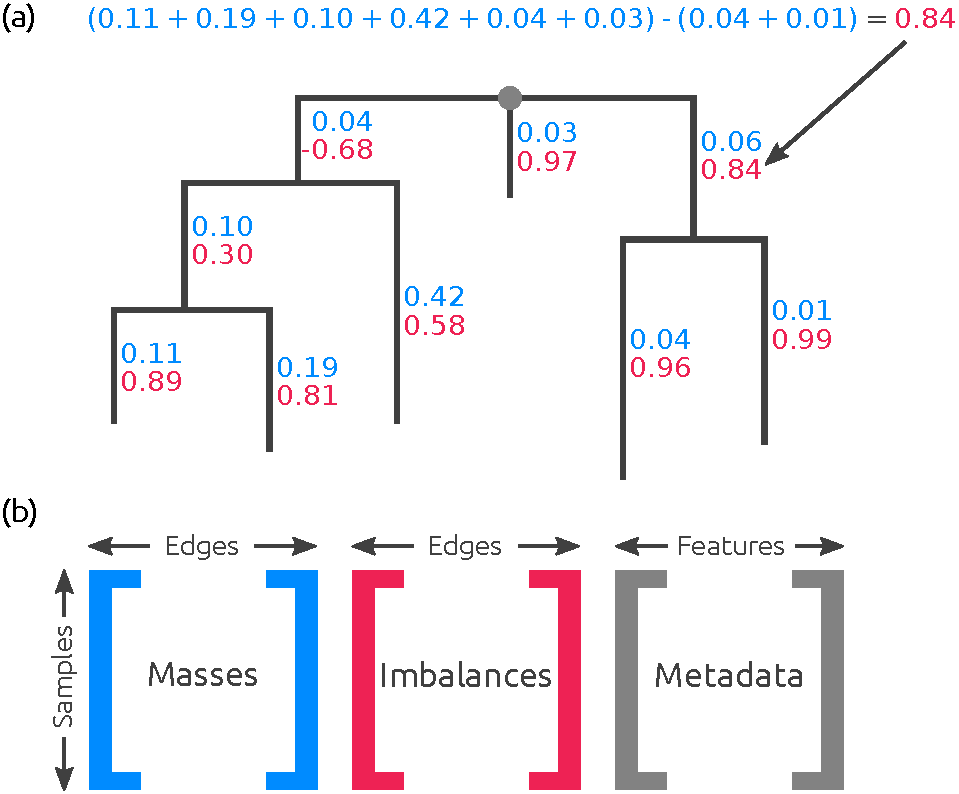
\includegraphics[width=0.8\linewidth]{imbalance.pdf}
    \begin{subfigure}{0pt}
        \phantomcaption
        \label{fig:imbalance:sub:ReferenceTree}
    \end{subfigure}
    \begin{subfigure}{0pt}
        \phantomcaption
        \label{fig:imbalance:sub:Matrices}
    \end{subfigure}
    \caption[Edge Masses and Imbalances]{
        \textbf{Edge Masses and Imbalances.}
        \subref{fig:imbalance:sub:ReferenceTree}
        Reference tree where each edge is annotated with the normalized mass (first value, blue) and
        imbalance (second value, red) of the placements in a sample.
        The imbalance is the sum of masses on the root side of the edge minus the sum of the masses on the non-root side.
        The depicted tree is unrooted, hence, its top-level trifurcation (gray dot) is used as ``root'' node.
        An exemplary calculation of the imbalance is given at the top.
        Because terminal edges only have a root side, their imbalance is not informative.
        \subref{fig:imbalance:sub:Matrices}
        The masses and imbalances for the edges of a sample constitute the rows of the first two matrices.
        The third matrix contains the available meta-data features for each sample.
        These matrices are used to calculate, for instance, the edge principal components or correlation coefficients.
    }
    \label{fig:imbalance}
\end{figure}

The key idea is to use the distribution of placement mass points over the edges of the \ac{RT} to characterize a sample.
This allows for normalizing samples of different size
by scaling the total sample mass to unit mass $1.0$.
In other words, absolute abundances are converted into relative abundances.
This way, rare species, which might have been removed by rarefaction, can be kept,
as they only contribute a negligible mass to the branches into which they have been placed.
This approach is analogous to using proportional values for methods based on OTU count tables,
that is, scaling each sample/column of the table by its sum of OTU counts \cite{Weiss2017}.
% In the following, we will mostly work with normalized samples.
Most of the methods presented here use normalized samples, that is, they use relative abundances.
As relative abundances are compositional data, certain caveats occur \cite{Aitchison1986,Lovell2015},
which we discuss where appropriate.

When working with large numbers of \acp{QS},
the mass interpretation allows to further simplify and reduce the data:
The masses on each edge of the tree can be quantized into $b$ discrete bins,
that is, each edge is divided into $b$ intervals (or bins) of the corresponding branch length.
All mass points on that edge are then accumulated into their respective nearest bin.
% , for example, at their nearest interval midpoint.
% Using midpoints means that masses are only minimally moved.
The parameter $b$ controls the resolution and accuracy of this approximation.
In the extreme case $b:=1$, all masses on an edge are grouped into one single bin.
This \emph{branch binning} process drastically reduces the number of mass points
that need to be stored and analyzed in several methods we present,
while only inducing a negligible decrease in accuracy.
As shown in \tabref{tab:hmp_binning_error}.
branch binning can yield a speedup of up to 75\% for post-analysis run-times.

Furthermore, using masses allows to summarize a set of samples
by annotating the \ac{RT} with their average per-edge mass distribution.
This procedure, also called \emph{squashing} \cite{Matsen2011a}, sums over all sample masses per edge
and then normalizes them once more to obtain unit mass for this resulting average tree.
This normalized tree thereby summarizes the (sub-)set of samples it represents.

% ======================================================================================================================
%     Edge Imbalances
% ======================================================================================================================

\subsection{Edge Imbalances}
\label{ch:Foundations:sec:PhylogeneticPlacementProcessing:sub:EdgeImbalances}

So far, we have only considered the per-edge masses.
Often, however, it is also of interest to ``summarize'' the mass of an entire clade. %, that is, to consider per-clade masses.
For example, sequences of the \ac{RT} that represent species or strains might not provide sufficient phylogenetic signal
for properly resolving the phylogenetic placement of short sequences \cite{Dunthorn2014}.
In these cases, the placement mass of a sequence can be spread across different edges representing the same genus or species,
thus blurring analyses based on per-edge masses.
% e.g., when using regions of the genome that lack the necessary phylogenetic signal for species delimitation.
% In that case, the distinction between masses on two related species branches ...
% it might be more useful to ``summarize'' the mass for the whole genus, that is, to consider per-clade masses.
% These masses then can be interpreted relative to the masses in the rest of the tree.
% The above visualizations show each edge individually, that is, they do not reveal information about whole clades.
Instead, a clade-based summary can yield clearer analysis results.
It can be computed by using the tree structure to appropriately transform the edge masses.
% The \acp{RT} used for phylogenetic placement are generally unrooted.
% They contain however a special node, the top-level trifurcation,
% which serves as a ``hook'' when drawing and storing the tree, and which we can consider as a root for simplicity.
Each edge splits the tree into two parts, of which only one contains the root (or top-level trifurcation) of the tree.
For a given edge, its mass difference is then calculated by summing all masses in the root part of the tree
and subtracting all masses in the other part,
while ignoring the mass of the edge itself \cite{Matsen2011a}.
% For a given edge, the edge mass difference is calculated as the difference between
% the sum of masses on the root side of the edge and all masses on the other side \cite{Matsen2011a}.
This difference is called the \emph{imbalance} of the edge.
It is usually normalized to represent unit total mass,
as the absolute (not normalized) imbalance otherwise propagates the effects of differing sample sizes all across the tree.
% doesn't matter where the root is, entries will change relative to each other accordingly when re-rooting
An example of the imbalance calculation is shown in \figref{fig:imbalance:sub:ReferenceTree}.
The edge imbalance relates the masses on the two sides of an edge to each other.
This implicitly captures the \ac{RT} topology and reveals information about its clades.
Furthermore, this transformation can also reveal differences in the placement mass distribution
of nearby branches of the tree.
This is in contrast to the KR distance, which yields low values for masses that are close to each other on the tree.
% This is for example useful when the tree contains taxa representing species or even strain level,
% which can often not be resolved using phylogenetic placement,
% e.g., when using regions of the genome that lack the necessary phylogenetic signal for species delimitation.
%Note that, %for normalized samples with unit total mass,
%the imbalance of a leaf edge is simply the total mass of the tree minus the mass of the edge.
% It thus contains mostly irrelevant information and can often be left out.
Examples that illustrate the different use cases for edge mass and edge imbalance metrics are shown in the Results section.

The edge masses and edge imbalances per sample can be summarized by two matrices,
which we use for all further downstream edge- and clade-related analyses, respectively.
In these matrices, each row corresponds to a sample, and each column to an edge of the \ac{RT}.
Note that these matrices can either store absolute or relative abundances,
depending on whether the placement mass was normalized.

Furthermore, many studies provide meta-data for their samples,
for instance, the pH value or temperature of the samples' environment.
Such meta-data features can also be summarized in a per-sample matrix, where each column corresponds to one feature.
The three matrices are shown in \figref{fig:imbalance:sub:Matrices}.
Quantitative meta-data features are the most suitable for our purposes,
as they can be used to detect correlations with the placement mass distributions of samples.
For example, Edge principal components analysis (Edge PCA) \cite{Matsen2011a}
is a method that utilizes the imbalance matrix to detect and visualize edges
with a high heterogeneity of mass difference between samples.
Edge PCA further allows to annotate its plots with meta-data variables, for instance, by coloring,
thus establishing a connection between differences in samples and differences in their meta-data \cite{Srinivasan2012}.
In the following, we propose several new techniques to analyze placement data and their associated meta-data.

% ======================================================================================================================
%     Distance between Samples
% ======================================================================================================================

\subsection{Distance between Samples}
\label{ch:Foundations:sec:PhylogeneticPlacementProcessing:sub:Distances}

kr distance. ref to nh distance?!
\cite{Evans2012}

% ======================================================================================================================
%     Existing Analysis Methods
% ======================================================================================================================

\subsection{Existing Analysis Methods}
\label{ch:Foundations:sec:PhylogeneticPlacementProcessing:sub:ExistingMethods}

squash clustering
edge pca
\cite{Matsen2011a,Evans2012}

we use these methods repeatedly to compare our novel methods to.
